\documentclass[12pt, a4paper, twoside]{article}
\usepackage[utf8]{inputenc}
\usepackage{fancyhdr}
\usepackage{graphicx}
\usepackage{caption}
\usepackage{subcaption}
\usepackage[margin=1in,footskip=0.25in]{geometry}
\usepackage{pgf}
\usepackage[absolute, overlay]{textpos}
\usepackage{pdfpages}
\usepackage[siunitx]{circuitikz}
\usepackage{adjustbox}

\setlength{\TPHorizModule}{1.0 pt}
\textblockorigin{\paperwidth}{0.0 pt}

\pagestyle{fancy}
\fancyhf{}
\lhead{Stromkreise \& Glühlampchen}
\rhead{Physik Bericht}
\begin{document}
    \pgfmathwidth{"\\\\ J. Dubois \& A. Huillet\\ MNG Rämibühl\\"}
    \begin{textblock}{\pgfmathresult}[1, 0](0, 0)
    \noindent
    \\\\ J. Dubois \& A. Huillet\\ MNG Rämibühl\\ 8001 Zürich
    \end{textblock}
    \begin{titlepage}

    \begin{center}
        \vspace*{8cm}
        \Huge
        \textbf{Stromkreise \& Glühlampchen}
 
        \vspace{0.5cm}
        \LARGE
        Physik Bericht  
    \end{center}
    \vspace*{8cm}
    \normalsize
    \hspace*{2cm}Physik Bericht mit Bezug auf das Praktikum vom 24. März 2022\\\\
    \hspace*{2cm}Zürich, 7. April 2022
    
             
 \end{titlepage}

    \newpage
    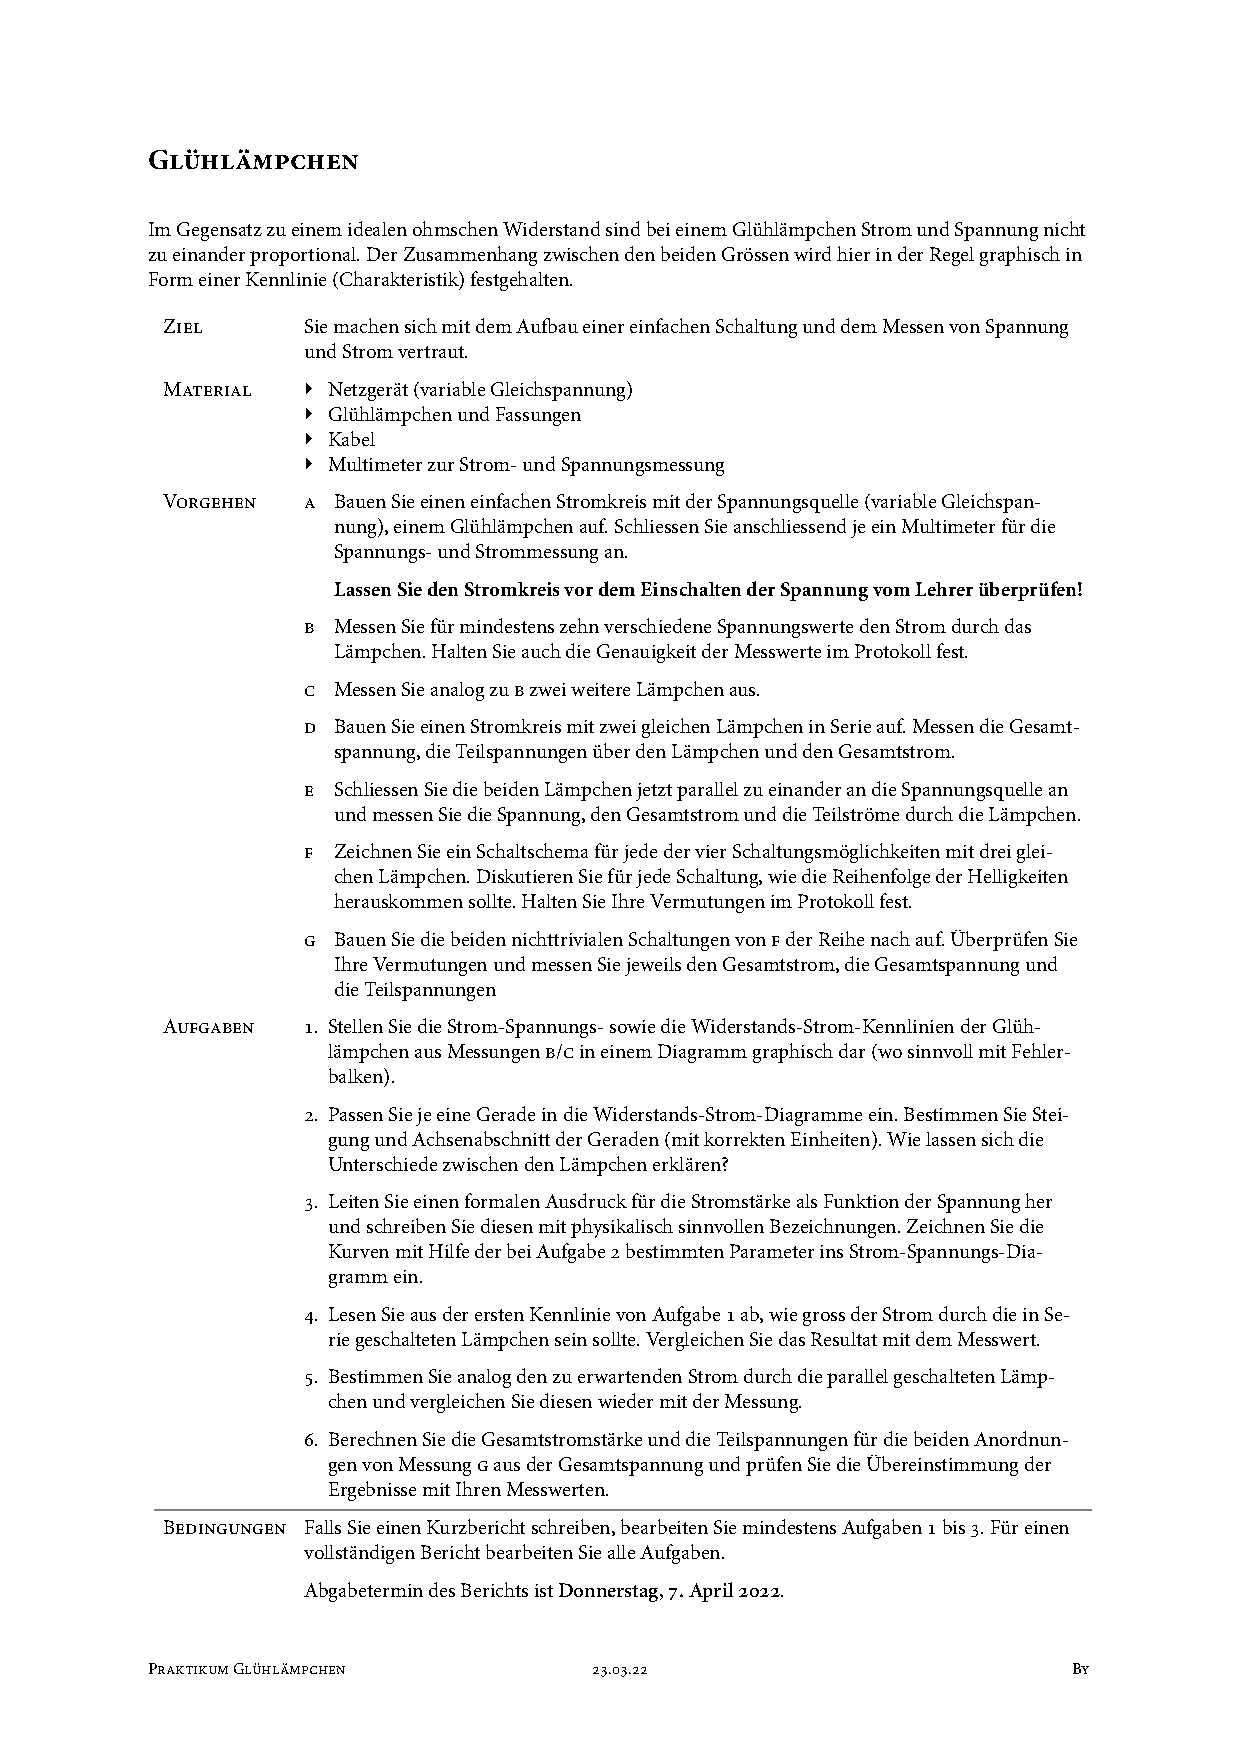
\includepdf[pages=-]{aufgabenstellung.pdf}
    \section{Einleitung}
    \newpage
    \section{Theorie}
    \newpage
    \section{Experiment}
    \newpage
    \section{Messungen}     
    \subsection{Messung A}
    Ein einfacher Stromkreis wurde gebaut. Dieser wird für die Messungen A, B und C\\ benutzt:\\
    \newline
    \begin{center}
        \begin{circuitikz} \draw
            (0,0) to[battery1, invert, l=\textit{U}] (0,4)
            to[lamp, i=\textit{I}] (4,4) -- (4,0) -- (0,0)
            ;
        \end{circuitikz}
    \end{center}
    \subsection{Messung B}
    Bei Messung B wurden für zehn verschiedenen Spannungswerte den Strom durch das Lämpchen gemessen:\\
    \begin{center}
        \begin{tabular}{l|r}
            \textbf{Spannung U[V]} & \textbf{Stromstärke I[mA]}\\
            \hline
            3.65 & 39.50\\
            5.11 & 48.30\\
            8.33 & 64.60\\
            10.37 & 73.60\\
            12.50 & 82.20\\
            15.54 & 93.60\\
            17.62 & 100.70\\
            19.74 & 107.70\\
            23.80 & 120.00\\
            24.85 & 123.00
        \end{tabular}
    \end{center}
    \newpage
    \subsection{Messung C}
    In dieser Messung wurde das gleiche Verfahren wie bei Messung B bei zwei weiter Lämpchen angewendet.\\\\
    \textbf{Messung für Lämpchen 2:}\\
    \begin{center}
        \begin{tabular}{l|r}
            \textbf{Spannung U[V]} & \textbf{Stromstärke I[mA]}\\
            \hline
            3.65 & 39.10\\
            5.11 & 48.40\\
            8.33 & 64.00\\
            10.37 & 73.30\\
            12.50 & 81.80\\
            15.54 & 93.60\\
            17.62 & 101.00\\
            19.74 & 107.90\\
            23.80 & 120.70\\
            24.85 & 123.90
        \end{tabular}
    \end{center}
    \vspace{1cm}
    \textbf{Messung für Lämpchen 3:}\\
    \begin{center}
        \begin{tabular}{l|r}
            \textbf{Spannung U[V]} & \textbf{Stromstärke I[mA]}\\
            \hline
            3.65 & 39.30\\
            5.11 & 48.50\\
            8.33 & 64.10\\
            10.37 & 73.30\\
            12.50 & 81.70\\
            15.54 & 93.40\\
            17.62 & 100.10\\
            19.74 & 107.10\\
            23.80 & 119.60\\
            24.85 & 122.80
        \end{tabular}
    \end{center}
    \subsection{Messung D}
    Folgender Stromkreis wurde aufgebaut:
    \begin{center}
        \begin{adjustbox}{scale=0.4}
        \begin{circuitikz} \draw
            (0,0) to[battery1, invert] (0,10)
            (0,10)--(16/3,10)
            (16/3,10)--(16/3,12)
            (16/3,10)--(16/3,8)
            (16/3,12) to[lamp, i=\textit{I1}] (32/3,12)
            (16/3,8) to[lamp, i=\textit{I2}] (32/3,8)
            (32/3,12)--(32/3,10)
            (32/3,8)--(32/3,12)
            (32/3,10)--(16,10)
            (16,10)--(16,0)--(0,0)
            ;
        \end{circuitikz}
    \end{adjustbox}
    \end{center}
    \subsection{Messung E}
    \subsection{Messung F}
    \subsection{Messung G}
    \newpage
    \section{Aufgaben}
    \newpage
    \section{Schlussfolgerungen}
    \newpage


\end{document}
